\chapter{Introduction}
\label{chap:intro}
\chaptoc{}

% ####################
\newpage
\section{Gravitational Waves}
\label{sec:gw}

\glspl{gw} are waves in space time.

\lipsum{}


% ~~~~~~~~~~~~~~~~~~~~
\subsection{Sources of gravitational waves}
\label{sec:gw-sources}

\lipsum{}


% ~~~~~~~~~~~~~~~~~~~~
\subsection{Detecting gravitational waves}
\label{sec:gw-detect}

\lipsum{}

% ~~~~~~~~~~~~~~~~~~~~
\subsection{Multi-messenger astronomy}
\label{sec:gw-multimessenger}

\lipsum{}


% ####################
\newpage
\section{The Gravitational-wave Optical Transient Observer}
\label{sec:goto}

The \gls{goto}\footnote{\url{https://goto-observatory.org/}} is a project dedicated to detecting future optical counterparts of gravitational wave sources by employing a wide-field approach to be able to localize such counterparts early. The first prototype instrument was inaugurated at the Roque de los Muchachos Observatory on La Palma, Canary Islands in July 2017 and is shown in Fig.~\ref{fig:goto_photo}. \gls{goto} uses arrays of \SI{40}{\cm} \glspl{ut} on a single fast-slewing mount. This modular approach allows the project to scale to large fields of view in a cost-effective manner. A full instrument will have 8 of these \glspl{ut} per mount, giving an overall field of view of \SI{40}{\square\deg} with a pixel scale of \SI[per-mode=symbol]{1.2}{\arcsec\per\pixel} and a limiting magnitude of \about20 in each two minute exposure. Each UT has a set of wide white and coloured filters to assist source characterisation.  An additional instrument with 8 more \glspl{ut} on a second mount is planned to be co-located in a second dome on La Palma, which will double the instantaneous field of view to \SI{80}{\square\deg}, allow the sky to be surveyed at a higher cadence and give more options for transient follow-up. A southern node is also planned for Australia.

\begin{figure}[htb]
\begin{center}
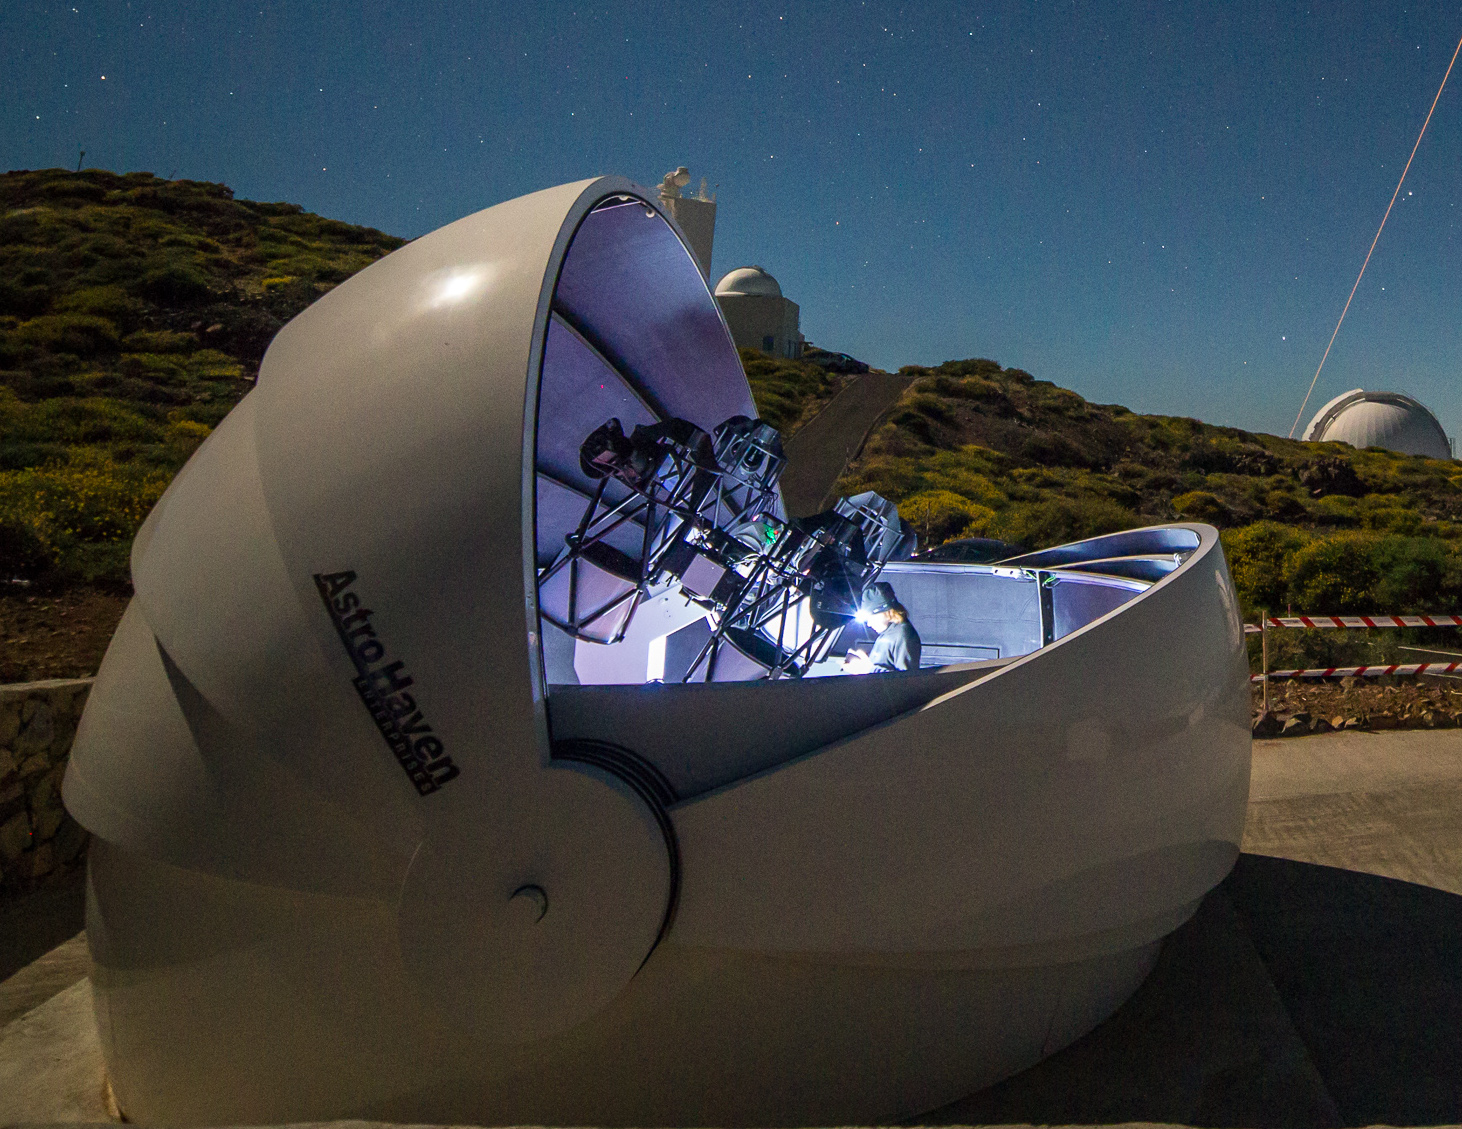
\includegraphics[width=11cm]{images/goto_photo.jpg}
\end{center}
\caption[The GOTO prototype instrument]{The GOTO prototype instrument on La Palma, with four of the eventual eight unit telescopes.}
\label{fig:goto_photo}
\end{figure}

\gls{goto} is designed as a robotic, wide-field transient detection telescope. Under normal circumstances the telescope will carry out an all-sky survey, based on a fixed grid of tiles. Each tile corresponds to the \SI{40}{\square\deg} field of view of the 8 \glspl{ut} observing neighbouring patches of sky, as shown in Fig.~\ref{fig:tiles}. The all-sky survey will aim to obtain a high-cadence at an appropriate depth, mapping the entire visible sky several times a week. The high cadence will ensure that there are very recent reference images available to allow detection of objects using difference imaging.

\begin{figure}[htb]
\begin{center}
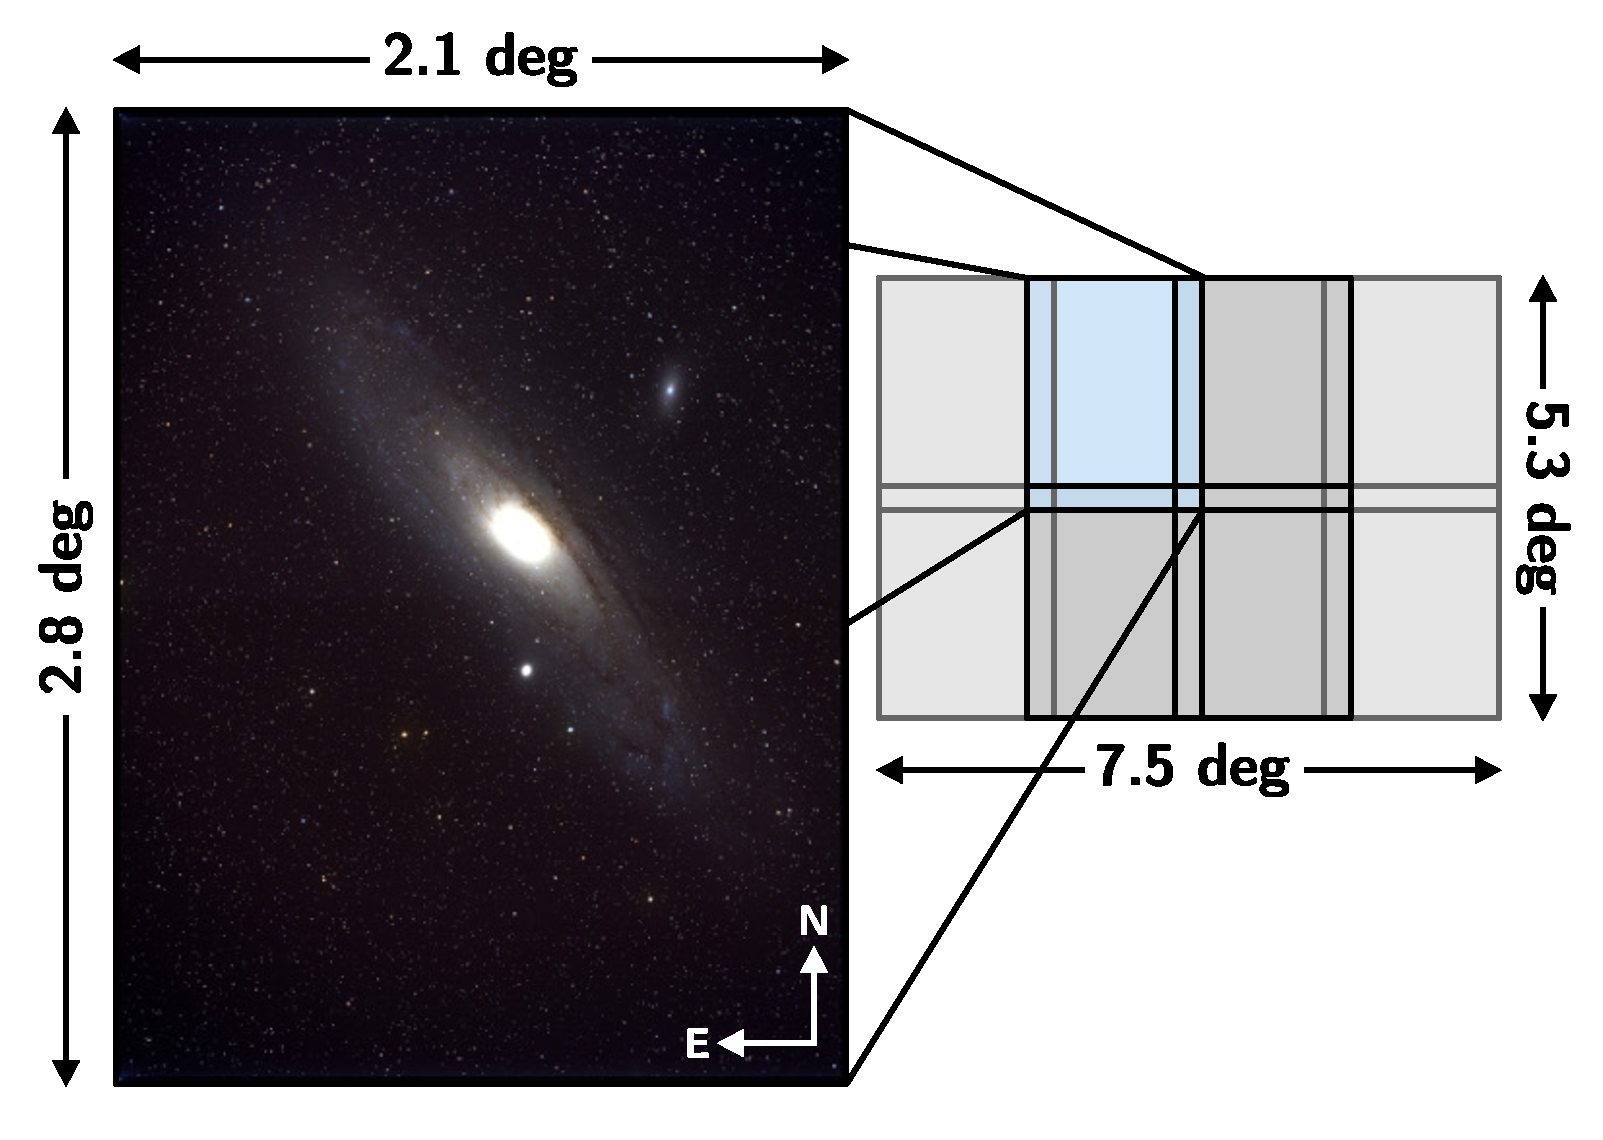
\includegraphics[width=11cm]{images/tiles.pdf}
\end{center}
\caption[M31]{A single commissioning image of M31, showing the wide field of view of each unit telescope. The full 8 unit telescope array will cover an area of approximately 40 square degrees, which forms a single survey tile.}
\label{fig:tiles}
\end{figure}

% ~~~~~~~~~~~~~~~~~~~~
\subsection{Motivation}
\label{sec:gw-motivation}

\lipsum{}

% ~~~~~~~~~~~~~~~~~~~~
\subsection{Design}
\label{sec:gw-design}

\lipsum{}
